% coding: utf-8
% --------------------------------------------------------------------------------------------------
% "Параметризация стабилизирующих управлений в стохастических системах с непрерывным временем", 2009
% : ядро
% --------------------------------------------------------------------------------------------------
\documentclass[12pt, a4paper, titlepage, openbib, oneside]{report}

\usepackage[utf8]{inputenc}
\usepackage[russian]{babel}
%\usepackage{indentfirst}
\usepackage{amsmath}
\usepackage{amssymb}
\usepackage{theorem}
\usepackage[russian]{varioref}
\usepackage[pdftex]{graphicx}
\usepackage{listings}

\frenchspacing
\fussy
\raggedbottom

\setlength{\leftmargin}{20mm}
\setlength{\rightmargin}{10mm}
\righthyphenmin=2
\emergencystretch=6pt


\newtheorem{teo}{Теорема}
\newtheorem{lemma}{Лемма}
\newtheorem{alg}{Алгоритм}
\newtheorem{df}{Определение}



\DeclareMathOperator{\diag}{\mathrm{diag}}





%\includeonly{abstract,toc,ch1,ch2,ch3,ch4,ch5,ch6,ch7,biblist}
\begin{document}

\renewcommand{\bibname}{Список использованной литературы}
\renewcommand{\chaptername}{Раздел}


\newcommand{\br}{\vspace{12pt}}
\newcommand{\eqdef}{\stackrel{\mathrm{def}}{=}}
\newcommand{\Rv}[1]{\mathbb{R}^{#1}}
\newcommand{\Rs}[2]{\mathbb{R}^{{#1} \times {#2}}}
\newcommand{\qed}{\vspace{12pt}\hfill \mbox{\raggedright \rule{.1in}{.1in}}}



% ---------------------------------------------------------------------------------------------
% Титульный лист
% ---------------------------------------------------------------------------------------------

\begin{titlepage}
	\begin{center}
		\par Федеральное агентство по образованию\vspace{0.7mm}
		\par Государственное образовательное учреждение\vspace{0.7mm}
		\par высшего профессионального образования\vspace{1.5mm}
		\par «Нижегородский Государственный университет им.~Н.\,И.\,Лобачевского»
		\vspace{1cm}
		{\fontsize{18pt}{9mm} \fontseries{bx} \selectfont
			\par Параметризация управлений
			\par в системах с марковскими переключениями\vspace{3mm}
			\par и задачах робастной стабилизации.
			%\par Приложение к задачам пассификации\vspace{3mm}
			%\par и робастной стабилизации.
		}
		\vspace{2cm}
		\par {\large Квалификационная работа бакалавра}
	\end{center}
	\vspace{2cm}
	\begin{tabbing}
		1-2-3-4-5-6-7-8-9-10-11-12\=-13-14-15-16-17-18-19-20-21-22-23-24-25\=-26-27-28-29 \kill
		{\fontsize{10pt}{10pt} \selectfont Выполнил:}                 \>                      \>                 \\
		{\fontsize{10pt}{10pt} \selectfont студент гр.~84--02}        \>                      \> {\fontsize{10pt}{10pt} \selectfont Архипов С.\,В.}  \\
		\\
		{\fontsize{10pt}{10pt} \selectfont Научный руководитель:}     \>                      \>                 \\
		{\fontsize{10pt}{10pt} \selectfont профессор, д.\,ф.--м.\,н.} \>                      \> {\fontsize{10pt}{10pt} \selectfont Пакшин П.\,В.}   \\
		\\
		{\fontsize{10pt}{10pt} \selectfont Заведующий кафедрой:}     \>                      \>                 \\
		{\fontsize{10pt}{10pt} \selectfont профессор, д.\,ф.--м.\,н.} \>                      \> {\fontsize{10pt}{10pt} \selectfont Федоткин М.\,А.}
	\end{tabbing}
	\vspace{3cm}
	\begin{center} {\fontsize{10pt}{3mm} \fontshape{sc} \selectfont
		Нижний Новгород \\
		2009 год
	} \end{center}
\end{titlepage}

\begin{abstract}
Целью работы является параметрическое описание (параметризация) динамических звеньев системы с обратной связью по состоянию, описываемую линейными уравнениями с непрерывным временем. Рассматриваются методы решения задачи построения управления, обеспечивающего экспоненциальную устойчивость замкнутой системы в среднеквадратическом смысле. Исследуются методы решения поставленной невыпуклой задачи как то $W$- и $P$-проблемы, исследуется их применение к классической задаче $\mathcal{H}_\infty$, анализируются достаточные условия разрешимости $W$- и $P$-проблем.

Полученные результаты переносятся на частный случай описания динамических звеньев системы с марковскими переключениями режимов работы, исследуется вопрос существования матрицы усиления, обеспечивающей экспоненциальную устойчивость в среднеквадратическом смысле. Изучаются вопросы одновременной и робастной стабилизации, даются алгоритмы решения поставленной задачи. Полученные результаты распространяются на проблему пассификации выхода динамической системы, дается описание метода исследования проблемы в этом случае.

Даются алгоритмы решения ряда невыпуклых задач с условиями их применимости, приводятся примеры.
\end{abstract}
 % +++
% coding: utf-8
% --------------------------------------------------------------------------------------------------
% "Параметризация стабилизирующих управлений в стохастических системах с непрерывным временем", 2009
% : содержание
% --------------------------------------------------------------------------------------------------

\tableofcontents % +++

% chapter 1: введение
\chapter*{Введение}
\addcontentsline{toc}{chapter}{Введение}

В настоящее время, проблема стабилизации обратной связи по выходу является одной из ключевых в современной теории управления. К сожалению, полностью она еще не решена, существуют лишь отдельные методы решения частных же задач. Проблема стабилизации обратной связи по выходу намного сложнее стабилизации по состоянию. Для последней проблемы уже существует хорошо разработанный математический аппарат\cite{BOYD} решения линейных матричных неравенств и уравнений, позволяющий получить решение либо точно, либо с достаточной точностью.

Широкое распространение получил \emph{линейно-квадратичный регулятор}\footnote{В англоязычной литературе принята аббревеатура \emph{LQR} (от \emph{Linear quadratic regulator\/})}~--- вид оптимального регулятора, использующего квадратичный функционал качества. Это задача, в которой динамическая система описывается линейными дифференциальными уравнениями, а показатель качества представляет собой квадратичный функционал, называется \emph{задачей линейно-квадратичного управления\/}. Общая постановка задачи такова: пусть у нас есть система дифференциальных уравнений и критерий оптимальности, описанные следующим образом

$$
\dot{x}=Ax+Bu{,}~~~~~J=\int_0^\infty \left( x^TQx + u^TRu \right)\,dt \longrightarrow \min\mbox{.}
$$

Известно\cite{BOYD}, что закон управления по отрицательной обратной связи должен иметь вид $u=-R^{-1}B^TPx$, где матрица $P$ находится из алгебраического уравнения Риккати:

$$
A^TP + PA - PBR^{-1}B^TP + Q = 0\mbox{.}
$$

Также широкое распространение получила задача \emph{линейно-квадратичного гауссовского управления}\footnote{Аналогично, в англоязычной литературые приняты аббревеатура \emph{LQG} и ее расшифровка~--- \emph{Linear quadratic Gaussian control}}~--- набор методов и математического аппарата теории управления для синтеза систем управления с отрицательной обратной связью для линейных систем с аддитивным гауссовским шумом. Синтез проводится путём минимизации заданного квадратичного функционала.

\begin{displaymath}
\left\{ \begin{array}{lcr}
         \dot{x}(t)& = & Ax(t) + Bu(t) + \xi(t)\mbox{,} \\
         y(t)& = &Cx(t) + Du(t) + \eta(t)\mbox{.}
        \end{array} \right.
\end{displaymath}
$$
J = \lim\limits_{T \to \infty} E \int\limits_0^T \left( x(t)^TRx(t) + u^T(t)Qu(t) \right)\,dt \longrightarrow \min\mbox{.}
$$

Где $\xi(t)$~--- возмущения, действующие на объект управления; $\eta(t)$~--- погрешность измерения. Матрицы $R$ и $Q$ представляют собой параметры функционала и являются положительно-определенными.\br

Основной целью работы является исследование задачи LQR-парамет\-ризации обратной связи по выходу для систем с непрерывным временем и марковскими переключениями. Основываясь на результатах исследования, предложены различные способы, методы и алгоритмы решения задачи. Полученные результаты могут быть непосредственно использованы при проектировании систем с помощью различных программных пакетов, как то MATLAB (с решателем YALMIP\footnote{ {\fontfamily{cmtt}\selectfont http://control.ee.ethz.ch/$\sim$joloef/wiki/pmwiki.php}. Автор пакета: Löfberg J. }), или с открытым пакетом SciLab (используя аналогичную наработку, SciYalmip\footnote{{\fontfamily{cmtt}\selectfont http://www.laas.fr/OLOCEP/SciYalmip/} Авторы пакета: Пакшин П., Соловьев С.}).\br

LQR-параметризация используется для синтеза систем управления. Проблема управляемости играет важную роль в адаптивных системах и заключается в следующем: должно существовать такое обратное управление и линейная комбинация вектора выхода $y$, вектора сигналов $\omega$ и соотвествующего ему вектора наблюдений $z$, такие, что замкнутая система будет также управляема относительно $z$. В современной теории управления достаточно хорошо изучен случай, когда $z=y$: в этом случае говорят о полной наблюдаемости. Однако, это все же достаточно жесткое ограничение, так как под него попадают лишь те системы, в которых число входов и выходов совпадает. Следующим шагом развития стало изучение случая, когда $z=Gy$ для заданной матрицы $G$. Очевидно, что это снимает ограничение на количество входов и выходов, однако вводит новую сложность~--- определение (если заранее неизвестна) $G$. Сравнительно хорошо изучен случай, когда $z=Gy+D\omega$~--- случай так называемого \emph{робастного адаптивного управления}.

Поиск такой матрицы $G$~--- задача весьма нетривиальная, представляющая сама собой достаточно сложный объект исследования. Решение, как правило, разбивают на 2 этапа: построение робастной стабилизирующей матицы усиления $F$; построение матрицы $G$ на базе полученной $F$. Сами по себе, эти задачи могут быть эффективно решены с помощью определенных матричных неравенств и уравнений. Однако условия, обеспечиваемые этими уравнениями, к сожалению, почти всегда являются достаточными, но никак не необходимыми. Следовательно, подходы не универсальны, применимы лишь для узкого класса задач. Впрочем, это никоим образом не снижает их высокой практической ценности.\br

Работа устроена следующим образом: в разделе 1 приведенная задача будет четко формализована. В разделе 2 будут предложены некоторые способы решения задачи, основанные на теоретических сведениях. В разделе 3 задача будет обобщена на линейные системы с марковскими переключениями в непрерывном времени, будут даны алгоритмы одновременной и робастной стабилизаций, основанные на теореме о матрице усиления. В разделе 4 полученные результаты будут перенесены на проблему наблюдаемости выхода. В разделе 5 будет показано практическое применение полученных результатов.
 % +++

% chapter 2: обзор задач
\chapter{Постановка основной задачи}

Пусть наша система с непрерывным временем задана следующей системой уравнений:

\begin{equation}
\label{eq:1/1}
\left\{ \begin{array}{rcl}
        \dot{x}&=&Ax + Bu\mbox{,} \\
        y&=&Cx\mbox{.}
       \end{array} \right.
\end{equation}

где $x=x(t)$, $x \in \Rv{n}$; $y=y(t)$, $y \in \Rv{n_y}$; $u=u(t)$, $u \in \Rv{n_u}$; $t \in [0, +\infty)$). Матрицы таковы, что $A \in \Rs{n}{n}$, $B \in \Rs{n_u}{n}$, $C \in \Rs{n_y}{n}$.

В 1890 году Ляпунов А.\,М. доказал, что система \vref{eq:1/1} стабилизируема тогда и только тогда, когда существуют положительно определенная матрица $P>0$\footnote{Здесь и далее выражение $M>0$ ($M<0$) означает положительную (отрицателную) определенность матрицы $M$} и $F$ подходящих размерностей такие, что выполняется неравенство:

\begin{equation}
\label{eq:1/2}
P(A-BF) + (A-BF)^TP < 0\mbox{.}
\end{equation}

Домножим \vref{eq:1/2} с обеих сторон на матрицу $W \eqdef P^{-1}$. Получаем:

\begin{equation}
\label{eq:1/3}
(A-BF)W + W(A-BF)^T < 0\mbox{.}
\end{equation}

Сделаем замену $L \eqdef FW$:

\begin{equation}
\label{eq:1/4}
AW + WA^T - LB - L^TB^T < 0\mbox{.}
\end{equation}

Получили известную задачу\cite{BOYD}, разрешимую в переменных $W$ и $L$ тогда и только тогда, когда пара матриц $A$ и $B$ будут устойчивыми. В этом случае управление определяется как $u=-LW^{-1}$. Проблема определения разрешимости может быть легко проделана засчет известных алгоритмов\cite{BOYD}. Например, можно использовать эллиминацию матричных переменных. Для этого нужно \vref{eq:1/4} переписать в виде

\begin{equation}
\label{eq:1/5}
AW + WA^T - \sigma BB^T < 0\mbox{.}
\end{equation}

Доказано, что $\sigma$ существует. Эквивалентой формой \vref{eq:1/5} является

$$
\hat{B}^T(AW+WA^T)\hat{B} < 0\mbox{,}
$$

\begin{flushleft}
где $\hat{B}$~--- ортогональное дополнение $B$. В этом случае оптимальное управление $F$ будет записано в виде
\end{flushleft}

\begin{equation}
\label{eq:1/6}
F = -\frac{\sigma}{2}B^TW^{-1}
\end{equation}

\begin{flushleft}
для любой $W>0$. Без ограничения общности можно полагать, что $\sigma=1$. В противном случае, всегда можно привести эквивалентные преобразования, в которых $\sigma$ <<исчезнет>>.\br
\end{flushleft}

Теперь предположим, что желаемая структура управления может быть записана в виде $u=-F_0y$ или, эквивалентно, $u=-Fx$. Очевидно, что $F \eqdef F_0C$. Тогда из \vref{eq:1/3} получаем:

\begin{equation}
\label{eq:1/7}
(A-BF_0C)W + W(A-BF_0C)^T < 0\mbox{,}~~~~~~W>0\mbox{.}
\end{equation}

Теоретическое решение задачи получено, однако оно не применимо на практике: это связано с тем, что неравенство относительно $W$ и $F_0$ не является в общем случае выпуклым, следовательно эффективные методы решения здесь не применимы. Впрочем, с использованием нескольких вспомогательных задач, являющихся выпуклыми, можно проблему в значительной мере упростить.
 % +++

% chapter 3: некоторые алгоритмы решения задачи
\chapter{Некоторые методы решения поставленных задач}

\section{$W$-проблема}

$W$-проблема тесно связана с \vref{eq:1/7} и формулируется следующим образом.

Пусть заданы некоторые матрицы $A$, $B$, $C$ (полагаем, что $C$ имеет полный строчный ранг). $W$-проблема заключается в нахождении матриц $W$, $N$ и $M$ таких, что

\begin{equation}
\label{eq:2/1}
\left\{ \begin{array}{l}
         AW + WA^T - BNC - C^TN^TB^T < 0\mbox{,} \\
         W > 0\mbox{,} \\
         MC = CW\mbox{.}
        \end{array}
\right.
\end{equation}

$W$-проблема вызывает двойной интерес. Во-первых, она выпукла, и, следовательно, может быть разрешена эффективными алгоритмами\cite{BOYD}, такими как эллиминация матричных переменных или $\mathcal{S}$-процедура (в частных случаях). Во-вторых, если она разрешима, то будет разрешимой и задача \vref{eq:1/7}.

Покажем это, доказав следующую теорему.

\begin{teo}
\label{teo:2/1}
Если $W$, $N$, $M$ являются решениями \vref{eq:2/1}, то управления

$$
u = -NM^{-1}y = -F_0y
$$

\begin{flushleft}
будут обеспечивать устойчивость системы \vref{eq:1/1}.
\end{flushleft}
\end{teo}

\emph{Доказательство}.
Так как $C$ имеет полный строчный ранг и выполняется условие $MC=CW$, то матрица $M$ также будет иметь полный строчный ранг. Следовательно, $C$ можно представить через уравнение

\begin{equation}
\label{eq:2/2}
C = M^{-1}CW\mbox{.}
\end{equation}

\begin{flushleft}
Примем $F_0 \eqdef -NM^{-1}$. Тогда подставляя \vref{eq:2/2} в \vref{eq:1/7}, после серии очевидных преобразований получим систему \ref{eq:2/1}.\qed
\end{flushleft}


% ----------------------------------------------------------------------


\section{$P$-проблема}

$P$-проблема практически идентична $W$-проблеме, так как получается из нее простой заменой переменных.

Пусть заданы матрицы $A$, $B$, $C$ подходящих размерностей. $B$ имеет полный строковый ранг. $P$-проблема заключается в нахождении, если это возможно, матриц $P$, $N$, $M$ таких, что

\begin{equation}
\label{eq:2/3}
\left\{ \begin{array}{l}
         PA + A^TP - C^TN^TB^T - BNC < 0\mbox{,} \\
         P > 0\mbox{,} \\
         BM = PB\mbox{.}
        \end{array}
\right.
\end{equation}

Совершенно аналогично доказывается теорема о $P$-проблеме.

\begin{teo}
\label{teo:2/2}
Если $P$, $N$, $M$ являются решениями $P$-проблемы \vref{eq:2/3}, то управления

$$
u = -N^{-1}My = -F_0y
$$

\begin{flushleft}
будут обеспечивать устойчивость системы \vref{eq:1/1}.
\end{flushleft}
\end{teo}

\emph{Замечание}. $P$- и $W$-проблемы схожи, так как представляют из себя разный взгляд на одни и те же уравнения. Если основой для $W$-проблемы служит уравнение \vref{eq:1/3}, то для $W$-проблемы~--- \vref{eq:1/2}.\br

Когда $C=E$\footnote{Здесь и далее, под $E$ понимается классическая единичная матрица подходящей размерности.} $W$-проблема значительно упрощается и сводится к стандартным техникам решения матричных неравенств вследствие того, что уравнение $MC=CW$ превращается в обычное равенство $M=W$. В этом случае $P$-проблема предоставляет альтернативные способы вычисления стабилизирующих матриц усиления обратной связи, которые могут представлять практический интерес в определенном классе задач\cite{CRUSIUS}.


% --------------------------------------------------------------------------------------------------



\section{Проблема $\mathcal{H}_\infty$}

$\mathcal{H}_\infty$-управление~--- метод теории управления для синтеза оптимальных регуляторов. Он является оптимизационным, имеющим дело со строгим математическим описанием предполагаемого поведения замкнутой системы и её устойчивости.

$\mathcal{H}$ является нормой в пространстве Харди\footnote{Расширение $\mathcal{L}^p$-пространства на комплексную плоскость.}. <<Бесконечность>> говорит о выполнении минимаксных условий в частотной области. $\mathcal{H}_\infty$~--- норма динамической системы, имеющая смысл максимального усиления системы по энергии.\br

Оказывается, что $W$- и $P$-проблемы могут быть использованы для решения $\mathcal{H}_\infty$-проблемы. Более того, результаты имеют настолько общий характер, что могут быть использованы и на $\mathcal{H}_2$ без потери выразительности.

Положим, что система описывается как

\begin{equation}
\label{eq:2/4}
\left\{ \begin{array}{l}
         \dot{x} = Ax + B_uu + B_\omega\omega\mbox{,} \\
         y = C_yx + D_{uy}u + D_{\omega y}\omega\mbox{,} \\
         z = C_zx + D_{uz}u + D_{\omega z}\omega\mbox{.}
        \end{array}
\right.
\end{equation}

\begin{flushleft}
Где $x$, $y$, $z$~--- вектора соответствующих размерностей. $A$, $B_u$, $B_\omega$, $C_y$, $D_{uy}$, $D_{\omega y}$, $C_z$, $D_{uz}$, $D_{\omega z}$~--- матрицы соответсвующих размерностей. Тогда справедлива связывающая теорема.
\end{flushleft}

\begin{teo}
\label{teo:2/3}
Пускай система описана с помощью \vref{eq:2/4}. $D_{uy}$, $D_{\omega y}$~--- нулевые матрицы. Введем обозначение:

$$
\Phi(W,N) \eqdef WA + A^TW - B_uNC_y - C^T_yN^TB^T_u\mbox{.}
$$

Предположим, что выполняется следующее матричное неравенство с ограничениями:

\begin{equation}
\label{eq:2/5}
\left\{
\begin{array}{l}
 \left( \begin{array}{ccc}
         \Phi(W,N)         & B_\omega     & WC^T_\omega - C^T_yN^TD^T_{uz} \\
         B^T_\omega        & -\gamma^2E   & D^T_{\omega z} \\
         C_zW - D_{uz}NC_y & D_{\omega z} & -E
        \end{array}
 \right) < 0\mbox{,} \\
MC_y=C_yW\mbox{,} \\
W > 0\mbox{.}
\end{array}
\right.
\end{equation}

Пусть \vref{eq:2/5} разрешимо относительно матриц $W$, $N$ и $M$. Если управление $u=-NM{-1}$, то для замкнутой относительно $\omega$ и $z$ системы норма $\mathcal{H}_\infty$ будет такой, что $\|G_{\omega z}\|_\infty < \gamma$.

\end{teo}

\emph{Доказательство}.
Известно\cite{BOYD}, что норма $\mathcal{H}_\infty$ будет меньше $\gamma$ тогда и только тогда, когда существует матрица $W>0$ такая, что

\begin{equation}
\label{eq:2/6}
\left( \begin{array}{ccc}
        WA^Tf+A_fW    & B_f           & WC^T_f \\
        B^T_f         & -\gamma^2E    & D^T_f \\
        C_fW          & D_f           & -E
       \end{array}
\right) < 0\mbox{,}
\end{equation}

где $A_f$, $B_f$, $C_f$ и $D_f$ представляют из себя матрицы пространства состояний исходной системы.

Применим к \vref{eq:2/4} управление $u=-F_0y$ и получим, что в этом конкретном случае $A_f = A-B_uF_0C_y$, $B_f = B_\omega$, $C_f = C_z - D_{uz}F_0C_y$ и $D_f = D_\omega$. Очевидно, что \vref{eq:2/6} выполняется при $A_f = A-B_uF_0C_y$ и $F_0 = NM^{-1}$. Совершенно аналогично доказательству теоремы \vref{teo:2/1} можно показать, что выполнение \vref{eq:2/6} влечет за собой и справедливость \vref{eq:2/5}. Следовательно, замкнутая система удовлетворяет требуемому условию $\|G_{\omega z}\|_\infty < \gamma$.\qed\br



% ------------------------------------------------------------------


\section{Анализ достаточности для $W$- и $P$-проблем}

Проблема разрешимости $W$- и $P$-проблем зависит от той интерпретации состояний, которую выбирают для описания динамической системы. Однако существуют преобразования, которые позволяют решить эти задачи, даже если это невозможно в изначальной интерпретации.

Пусть $x$ определяет вектор состояния системы \vref{eq:1/1}. Преобразуем систему следующим образом: $x_0 = T_0^{-1}x$. Определим $T$ как $T \eqdef T_0T_0^T$ и произведем замену матриц ($A$, $B$, $C$, $P$, $W$) на ($T_0^{-1}AT_0$, $T_0^{-1}B$, $CT_0$, $T_0^TPT_0$, $T_0W{T_0^{-1}}^T$). Тогда \vref{eq:2/1} и \vref{eq:2/3} перепишутся следующим образом:

\begin{equation}
\label{eq:2/7}
\left\{ \begin{array}{l}
AW + WA^T - BNCT - TC^TN^TB^T < 0\mbox{,} \\
MCT = CW\mbox{,} \\
W > 0\mbox{,} \\
T > 0\mbox{;}
\end{array} \right.
\end{equation}

\begin{equation}
\label{eq:2/8}
\left\{ \begin{array}{l}
PA + A^TP - C^TN^TB^TT^{-1} - T^{-1}BNC < 0\mbox{,} \\
T^{-1}BM = PB\mbox{,} \\
P > 0\mbox{,} \\
T^{-1} > 0\mbox{.}
\end{array} \right.
\end{equation}

Совершенно очевидно, что после подобных преобразований $W$- и $P$-проблемы могут стать разрешимыми, даже если в исходных пространствах они таковыми не являлись. Но, к сожалению, \vref{eq:2/7} и \vref{eq:2/8} не являются выпуклыми относительно ($W$, $N$, $M$, $T$) и ($P$, $N$, $M$, $T^{-1}$) соотвественно. Задача определения преобразования, после которого исходные задачи станут разрешимыми до сих пор является открытой.

Впрочем, можно отметить тот немаловажный факт, что $W$-проблема инвариантна относительно преобразований $T_0$, удовлетворяющих уравнению $CT=RC$ для некоторой матрицы $R$ и $T\colon~T=T_0T_0^T$: это следует из \vref{eq:2/7}, где можно провести обычную замену переменных $N$ и $M$, сводящих уравнение к аналогичному. Аналогичный факт устанавливается и для $P$-проблемы: она будет инвариантна относительно преобразования $T_0$, которое удовлетворяет уравнению $T^{-1}B=BR$. Очевидным примером такого преобразования является $T \equiv E$ (ортогональные преобразования $T_0T^T_0=E$).

Хорошо известен\cite{PERES} следующий факт.

\begin{teo}
\label{teo:2/4}
Система \vref{eq:1/1} стабилизируема обратной связью по состоянию тогда и только тогда, когда существует подобное преобразование, что $C=(I~~~0)$ и \vref{eq:1/4} разрешима с $W$ и $L$, удовлетворяющим следующим структурным ограничениям:

\begin{eqnarray*}
W&=&\left( \begin{array}{cc}
            W_1 &   0 \\
            0   & W_2
           \end{array} \right)\mbox{,} \\
L&=&\left( L_1~~~0 \right)\mbox{.}
\end{eqnarray*}

\end{teo}

Отметим, что $C=(I~~~0)$ и ограничение $MC=CW$ в \vref{eq:2/1} эквивалентны тому, что $W$ имеет такую структуру. Если взять $L=(N~~~0)$, то можно показать\cite{PERES}, что система \vref{eq:1/1} стабилизируема через обратную связь по состоянию тогда и только тогда, когда существует преобразование подобия, превращающее $W$-проблему в разрешимую.\br

Аналогичные рассуждения справедливы и при рассмотрении $P$-проб\-лемы.
 % +++

% chapter 4: линейные системы с марковскими переключениями
\chapter[Параметризация в стохастических системах]{Параметризация стабилизирующих управлений в стохастических системах}

В этом разделе будет рассмотрено расширение задачи \vref{eq:1/1} на случай стохастических систем. Рассматривается частный случай, при котором система имеет марковские переключения режимов работы. Предыдущие методы~--- $W$- и $P$-проблемы~--- распространяются и на такую модификацию с незначительными изменениями, однако ввиду сужения области исследования, становится возможным использовать и несколько иные подходы, представляющие из себя законченные алгоритмы. Подробнее они будут исследованы в разделе 4. Целью этого же раздела является формализация расширенной задачи и некоторые ценные теоретические сведения, являющиеся основой для дальнейшей работы.\br


% ------------------------------------------------------------------------------------------------------


\section{Формализация задачи}

Задачу \vref{eq:1/1} на случай стохастических систем можно расширить следующим образом. Положим, что система с марковскими переключениями описывается следующей системой уравнений:

\begin{equation}
\label{eq:3/1}
\left\{ \begin{array}{l}
\dot{x}(t) = A\left(r(t)\right)x(t) + B\left(r(t)\right)u(t)\mbox{,} \\
y(t) = C\left(r(t)\right)x(t)\mbox{.}
\end{array} \right.
\end{equation}

Здесь $x(t) \in \Rv{n}$~-- вектор состояний динамической системы; $y(t) \in \Rv{k}$~--- вектор выхода динамической системы; $u(t) \in \Rv{m}$~--- вектор управлений. Матрицы $A$, $B$ и $C$ имеют соответствующие размерности. $r(t)$~($t~\geqslant~0$)~--- процесс переключений режимов работы, принимающий значения из конечного множества $\mathbb{N} = \left\{1,2, \ldots, N\right\}$. Этот процесс моделируется однородной марковской цепью с вероятностями переходов

\begin{eqnarray}
\label{eq:3/2}
\mathbf{P}\big(r(t+h) = j~|~r(t) = i \big) = \left\{ \begin{array}{lr}
\pi_{ij} + o(h) & \mbox{при } i \not= j\mbox{,} \\
1 + \pi_{ij} + o(h) & \mbox{при } i=j\mbox{;}
\end{array} \right. \\
i,j = 1,2,\ldots,N\mbox{.} \nonumber
\end{eqnarray}

Вероятность $\pi_{ij}>0$~--- вероятность переключения из режима $i$ в момент времени $t$ в режим $j$ в момент времени $t+h$ (полагаем $h>0$). Из определения \vref{eq:3/2} и свойств вероятностей следует, что $\pi_{ii} = -\sum_{i\not=j}^N\pi_{ij}$ ($i,j=1,2,\ldots,N$). То обстоятельство, что $\pi_{ii}<0$ не является существенным, так как является чисто конструктивной особенностью и может быть легко исправлено\cite{CDC} (что приведет к усложнению математических выкладок, но лишь по части их громоздкости).

Аналог матрицы вероятностей переходов в марковской цепи~--- матрица $\Pi \eqdef \|\pi_{ij}\|_{\left\{i,j=1,2,\ldots,N\right\}}$.\br

Закон управления с обратной связью определяется совершенно аналогично:

\begin{equation}
\label{eq:3/4}
u(t)=F_iy(t) \mbox{~при } r(t)=i\mbox{.}
\end{equation}

Задача поставлена.



% ------------------------------------------------------------------------------------------------------



\section{Теорема о существовании матрицы усиления}

Будет рассмотрена и доказана теорема, которая дает основные теоретические результаты, на базе которых будут строиться методы решения задачи \vref{eq:3/1} в следующем разделе. Эта теорема основывается на LQR-концепциях и расширяет уже имеющиеся сведения\cite{GLXKA}, касаемые класса систем с марковскими переключениями.

\begin{teo}
\label{teo:3/1}
Матрица усиления $F_i$, обеспечивающая экспоненциальную устойчивость систем \ref{eq:3/1}-\ref{eq:3/4} в среднеквадратическом смысле, существует тогда и только тогда, когда найдутся такие матрицы параметров $Q_i\colon~Q_i = Q_i^T \geqslant 0$ и $R_i\colon~R_i = R_i^T \geqslant 0$, что будет выполнено следующее матричное уравнение:

\begin{equation}
\label{eq:3/5}
F_iC = R_i^{-1}[B_i^TH_i + L_i]\mbox{.}
\end{equation}

Матрицы $H_i\colon~H_i = H_i^T > 0$ и $L_i$ ($L_i \in \mathbb{N}$) есть решения следующей системы матричных неравенств:

\begin{eqnarray}
\label{eq:3/6}
\left\{ \begin{array}{l}
A_i^TH_i + H_iA_i - H_iB_iR_i^{-1}B_i^TH_i + Q_i \\
+ \sum\limits_{i=1}^N\pi_{ij}H_j + L_i^TR_i^{-1}L_i < 0\mbox{,}
\end{array} \right. \\
i \in \mathbb{N}\mbox{.} \nonumber
\end{eqnarray}

\end{teo}

\emph{Необходимость}.
Пусть $F_i$~--- искомая матрица усиления. Тогда будет существовать\cite{KM} положительно определенное решение $H_i\colon~H_i = H_i^T$ следующей системы неравенств:

$$
A_{ci}^TH_i + H_iA_{ci} + \sum\limits_{i=1}^N\pi_{ij}H_j + Q_i + (F_iC_i)^TR_iF_iC_i < 0\mbox{,}~~~~i \in \mathbb{N}\mbox{,}
$$

где $A_{ci} \eqdef A_i - B_iF_iC_i$, $Q_i = Q_i \geqslant 0$ и $R_i = R_i^T \geqslant 0$. После перегруппировки слагаемых, получаем, что

\begin{eqnarray}
\label{eq:3/7}
A_i^TH_i + H_iA_i + (F_iC_i)^TR_iC_iF_i - (F_iC_i)^TB_iH_i - \nonumber \\
H_iB_iF_iC_i + \sum\limits_{i=1}^N\pi_{ij}H_j + Q_i < 0\mbox{,}~~~~i \in \mathbb{N}\mbox{.}
\end{eqnarray}

Положим

\begin{equation}
\label{eq:3/8}
K_i \eqdef F_iC_i - R_i^{-1}B^T_iH_i\mbox{.}
\end{equation}

Перепишем \vref{eq:3/7} в следующей форме:

\begin{eqnarray}
\label{eq:3/9}
A_i^TH_i + H_iA_i - H_iB_iR_i^{-1}B_i^TH_i + \nonumber \\
K_i^TR_iK_i + \sum\limits_{i=1}^N\pi_{ij}H_j + Q_i < 0\mbox{.}
\end{eqnarray}

Затем положим

\begin{equation}
\label{eq:3/10}
L_i \eqdef R_iK_i\mbox{.}
\end{equation}

Подставляя \vref{eq:3/10} в \vref{eq:3/9} и учитывая, что $FC$~--- константная матрица, непосредственно получаем \vref{eq:3/5} и \vref{eq:3/6}.\br

\emph{Достаточность}.
Пускай существуют матрицы $H_i\colon~H_i = H_i^T$ и $F_i$, удовлетворяющие \vref{eq:3/5} и \vref{eq:3/6}. Определим матрицы $K_i$ и $L_i$ такими же, как  в \vref{eq:3/8} и \vref{eq:3/10} соотвественно. Тогда справедливо, что

\begin{eqnarray}
\label{eq:3/11}
0 > A_i^TH_i + H_iA_i - H_iB_iR_i^{-1}B_i^TP_i + \nonumber \\
\sum\limits_{i=1}^N\pi_{ij}H_j + L_i^TR_iL_i + Q_i = \nonumber \\
(A_i - B_iF_iC_i)^TH_i + H_i(A_i - B_iF_iC_i) + \nonumber \\
\sum\limits_{i=1}^N\pi_{ij}H_j + (F_iC_i)^TR_iF_iC_i + Q_i\mbox{,}~~~i \in \mathbb{N}\mbox{.}
\end{eqnarray}

Откуда следует справедливость \vref{eq:3/7}, следовательно $F_i$~--- искомая матрица усиления.\qed\br
 % +++

% chapter 5: алгоритмы решения задач
\chapter{Методы решения задачи LQR-параметризации}

Теорема \vref{teo:3/1} дает основной теоретический результат, лежащий в основе всех методов решения задачи LQR-параметризации в линейных системах с непрерывным временем и марковскими переключениями. Следует, однако, отметить тот факт, что почти все они носят достаточный характер, не являясь необходимыми. Поэтому если вдруг один подход не срабатывает, то это вовсе не означает, что задача не решаемая, следует попробовать их все. И даже в том случае, если ни один из них не сработает, определенно утверждать неразрешимость задачи все равно нельзя.

Проблема решения усугубляется еще и тем, что \ref{eq:3/5} и \vref{eq:3/7} не являются стандартными выпуклыми матричными неравенствами.



% --------------------------------------------------------------------------------------------------------------



\section{Метод достаточных выпуклых условий}

Так как \ref{eq:3/5} и \vref{eq:3/7} являются нестандартными матричными неравенствами, которые, к тому же, не выпуклы, то обычные методы и алгоритмы решения не подходят. Возникает идея построения серии вспомогательных выпуклых задач, зная решение которых, требуемую матрицу усиления $F_i$ все же можно построить.

Положим

\begin{eqnarray*}
X_i \eqdef H_i^{-1}{,~~~~} Y_i \eqdef L_iX_i\mbox{,} \\
\Lambda_{11i} \eqdef X_iA_i^T + A_iX_i + \pi_{ii}X_i - B_iR_i^{-1}B_i\mbox{,} \\
\Lambda_{12i} \eqdef X_i\sqrt{Q_i}\sqrt{\pi_{i1}}X_i \cdots \sqrt{\pi_{i\,i-1}}X_i\sqrt{\pi_{i\,i+1}}X_i \cdots \sqrt{\pi_{iN}}X_iY_i^T\mbox{,} \\
\Lambda_{22i} \eqdef \diag[-E~-X_1 \ldots -X_{i-1}~-X_{i+1} \ldots -X_N~-R_i]\mbox{.}
\end{eqnarray*}

В этом случае можно переписать \ref{eq:3/5} и \vref{eq:3/7} в виде матричного неравенства

\begin{equation}
\label{eq:4/1}
\left[ \begin{array}{lr}
    \Lambda_{11i}   & \Lambda_{12i} \\
    \Lambda^T_{12i} & \Lambda_{22i}
\end{array} \right] > 0\mbox{,}~~~i \in \mathbb{N}\mbox{.}
\end{equation}

\begin{equation}
\label{eq:4/2}
F_iC_iX_i = R_i^{-1}(B^T_i + Y_i)\mbox{,}~~~i \in \mathbb{N}\mbox{.}
\end{equation}

Из определения $P$-проблемы \ref{eq:2/3} и теоремы \vref{teo:2/2} следует, что существуют такие матрицы $M_i$ ($i \in \mathbb{N}$), что

\begin{equation}
\label{eq:4/3}
C_iX_i = M_iC_i\mbox{,}~~~i \in \mathbb{N}\mbox{.}
\end{equation}

Тогда \vref{eq:4/2} разрешимо относительно $F_i$ тогда и только тогда\cite{SIG}, когда

\begin{equation}
\label{eq:4/4}
(B_i^T + Y_i)(E - C_i^+\footnote{Под $C^+_i$ понимается псевдообращение матрицы $C_i$ по Муру-Пенроузу.}C_i) = 0\mbox{,}~~~i \in \mathbb{N}\mbox{.}
\end{equation}

Все решения \vref{eq:4/2} непосредственно записываются в виде

\begin{equation}
\label{eq:4/5}
F_i = [R_i^{-1}(B_i^T+Y_i)C^+_i+Z_i(E+C_i^+C_i)]M_i^{-1}\mbox{,}~~~i \in \mathbb{N}\mbox{,}
\end{equation}

где $Z_i$ ($i \in \mathbb(N)$)~--- произвольная матрица подходящей размерности.\br

Следовательно, для некоторых матриц $Q_i\colon~Q_i = Q_i^T \geqslant 0$, $R_i\colon~R_i = R_i^T > 0$ система совокупных линейных уравнений и неравенств \ref{eq:4/1}-\vref{eq:4/3} относительно переменных $X_i$, $Y_i$ и $M_i$ ($i \in \mathbb{N}$) разрешима. Закон управления \vref{eq:3/4} с матрицами усиления, заданными \vref{eq:4/5} будет обеспечивать экспоненциальную устойчивость в среднеквадратическом смысле системы \vref{eq:3/1}.

Можно предложить алгоритм, основанный на приведенных выше рассуждениях.

\begin{alg}
\label{alg:4/1} Метод достаточных выпуклых условий.
\begin{enumerate}
\item Зададим матрицы $Q_i$ и $R_i$, основываясь на LQR-условиях и разрешим задачи \ref{eq:4/1} и \ref{eq:4/3} относительно переменных $X_i$, $Y_i$ и $M_i$ ($i \in \mathbb{N}$);
\item Если задача на шаге 1 разрешима, то вычисляем матрицу усиления $F_i$ по формуле \vref{eq:4/5} для произвольной $Z_i$ ($i \in \mathbb{N}$).
\end{enumerate}

\end{alg}



% --------------------------------------------------------------------------------------------------------------



\section{Метод решения задачи одновременной стабилизации}

Задача одновременной стабилизации получается как частный случай \ref{eq:3/1}-\vref{eq:3/4} при $F_i \equiv F$ и $\pi_{ij}=0$ ($i,j \in \mathbb{N}$). Тогда система \vref{eq:3/1} перепишется в виде

\begin{eqnarray}
\label{eq:4/6}
\left\{ \begin{array}{l}
\dot{x}(t) = A_ix(t) + B_iu(t)\mbox{,} \\
y(t) = Cx(t)\mbox{;}
\end{array} \right. \\
i \in \mathbb{N}\mbox{,} \nonumber
\end{eqnarray}

а обратная связь как

\begin{equation}
\label{eq:4/7}
u(t) = -Fy(t)\mbox{.}
\end{equation}

Матрица усиления $F$ системы \ref{eq:4/6}-\vref{eq:4/7}, которая обеспечивает экспоненциальную устойчивость в среднеквадратическом смысле, существует тогда и только тогда, когда найдутся матрицы $Q_i\colon~Q_i = Q_i^T \geqslant 0$, $R_i\colon~R_i = R_i^T > 0$, что справедливо уравнение

\begin{equation}
\label{eq:4/8}
FC = R_i^{-1}[B_i^TH_i + L_i]\mbox{,}~~~i \in \mathbb{N}\mbox{.}
\end{equation}

Очевидно, что это уравнение суть преобразованное \ref{eq:3/5} для частного случая. Здесь $H_i\colon~H_i = H_i^T > 0$, а $L_i$ ($i \in \mathbb{N}$)~--- решение системы матричных неравенств

\begin{equation}
\label{eq:4/9}
A_i^TH_i + H_iA_i - H_iB_iR_i^{-1}B_i^TH_i + Q_i + L_i^TR_i^{-1}L_i < 0\mbox{,}~~~ i \in \mathbb{N}\mbox{.}
\end{equation}

Тогда для вычисления матрицы усиления можно предложить алгоритм, сходный решению $\mathcal{H}_\infty$-проблемы с помощью теоремы \vref{teo:2/3}.

\begin{alg}
\label{alg:4/2}
Метод решения задачи одновременной стабилизации.

\begin{enumerate}
\item Положим матрицы $Q_i\colon~Q_i = Q_i^T \geqslant 0$ и $R_i\colon~R_i = R_i^T > 0$, основываясь на LQR-соображениях, и решим следующие матричные неравенства и уравнения относительно переменных $X_i$, $Y_i$, $M_i$ ($i \in \mathbb{N}$) и $K$:
\begin{eqnarray}
\label{eq:4/10}
\left\{ \begin{array}{l}
         \left( \begin{array}{ccc}
                 X_iA_i^T + A_iX_i - B_i^TR_i^{-1}B_i  &  X_i\sqrt{Q_i}  &  Y_i^T \\
                 \sqrt{Q_i}X_i   &   -E   &   0 \\
                 Y_i   &   0   &   -R_i
                \end{array}
         \right) < 0\mbox{,} \\
         CX_i = M_iC\mbox{,} \\
         K \eqdef R_i^{-1}(B_i^T + Y_i)\mbox{,} \\
         (B_i^T + Y_i)(E - C_i^+C_i) = 0\mbox{;}
        \end{array} \right. \\
i \in \mathbb{N}\mbox{.} \nonumber
\end{eqnarray}

\item Если \vref{eq:4/10} разрешима, то вычислим матрицу усиления обратной связи $F$ по следующей формуле:

\begin{equation}
\label{eq:4/11}
F = [R_i^{-1}(B_i^T + Y_i)C_i^+ + Z(E + C_i^+C_i)]M_i^{-1}\mbox{.}
\end{equation}

для произвольных $i \in \mathbb{N}$ и матриц параметров $Z$.

\end{enumerate}

\end{alg}




% --------------------------------------------------------------------------------------------------------------



\section{Метод решения задачи робастной стабилизации}

Рассмотрим еще более частный случай задачи \vref{eq:4/6}. Примем, что пара матриц $(A_i,B_i)$ предствляют собой грани политопа, а $H_i = H_i^T \equiv H > 0$. Эта задача является проблемой робастой устойчивости с политопической неопределенностью

\begin{eqnarray}
\label{eq:4/12}
\left\{ \begin{array}{l}
\dot{x} = \sum\limits_{i=1}^N \xi_i(t)[A_ix(t) + B_iu(t)]\mbox{,} \\
y(t) = Cx(t)
\end{array} \right. \\
i \in \mathbb{N}\mbox{,} \nonumber
\end{eqnarray}

где $\xi_i(t) \geqslant 0$ и $\sum_{i=1}^N\xi_i(t)=1$. Обратная связь, как и в \vref{eq:4/7}, представляется в виде $u(t) = Fy(t)$.\br

Утверждается, что матрица усиления обратной связи $F$ будет обеспечивать экспоненциальную устойчивость системы \vref{eq:4/12}-\ref{eq:4/7} в среднеквадратическом смысле тогда и только тогда, когда найдутся матрицы параметров $Q_i\colon~Q_i = Q_i^T \geqslant 0$ и $R_i\colon~R_i = R_i^T > 0$, такие, что выполняется уравнение, аналогичное \vref{eq:4/8}:

\begin{equation}
\label{eq:4/13}
FC = R_i^{-1}[B_i^TH + L_i]\mbox{,}~~~i \in \mathbb{N}\mbox{.}
\end{equation}

где $L_i$~--- решение соответствующей системы матричных неравенств:

\begin{equation}
\label{eq:4/14}
A_i^TH + HA_i - HB_iR_i^{-1}B_i^TH + Q_i + L_i^TR_i^{-1}L_i < 0\mbox{,}~~~ i \in \mathbb{N}\mbox{.}
\end{equation}

Основываясь на этих результатах, предлагается алгоритм, схожий с алгоритмом \vref{alg:4/2}.

\begin{alg}
\label{alg:4/3}
Метод решения задачи робастной стабилизации.

\begin{enumerate}
\item Положим матрицы $Q_i\colon~Q_i = Q_i^T \geqslant 0$ и $R_i\colon~R_i = R_i^T > 0$, основываясь на LQR-соображениях, и решим следующие матричные неравенства и уравнения относительно переменных $X_i$, $Y_i$, $M_i$ ($i \in \mathbb{N}$) и $K$:
\begin{eqnarray}
\label{eq:4/15}
\left\{ \begin{array}{l}
         \left( \begin{array}{ccc}
                 X_iA_i^T + A_iX_i - B_i^TR_i^{-1}B_i  &  X_i\sqrt{Q_i}  &  Y_i^T \\
                 \sqrt{Q_i}X_i   &   -E   &   0 \\
                 Y_i   &   0   &   -R_i
                \end{array}
         \right) < 0\mbox{,} \\
         CX_i = M_iC\mbox{,} \\
         K \eqdef R_i^{-1}(B_i^T + Y_i)\mbox{,} \\
         (B_i^T + Y_i)(E - C^+C) = 0\mbox{;}
        \end{array} \right. \\
i \in \mathbb{N}\mbox{.} \nonumber
\end{eqnarray}

\item Если \vref{eq:4/15} разрешима, то вычислим матрицу усиления обратной связи $F$ по следующей формуле:

\begin{equation}
\label{eq:4/16}
F = [R_i^{-1}(B_i^T + Y_i)C^+ + Z(E + C^+C)]M_i^{-1}\mbox{.}
\end{equation}

для произвольных $i \in \mathbb{N}$ и матриц параметров $Z$.

\end{enumerate}

\end{alg}



% --------------------------------------------------------------------------------------------------------------


\pagebreak
\section{Итерационный алгоритм}

Из теоремы \vref{teo:3/1} непосредственно следует итерационный алгоритм, основной идеей которого является последовательное вычисление последовательности матриц $P_n$, которое должно сходится к требуемой матрице.

\begin{alg}
\label{alg:4/4}

Итерационный алгоритм.

\begin{enumerate}

\item
Задаем некоторые произвольные $Q\colon~Q=Q^T>0$ и $R\colon~R=R^T>0$. Полагаем $n=0$, $L_0=0$. Решаем систему билинейных матричных неравенств относительно $P=P^T>0$ и $K$.

\begin{eqnarray}
\label{eq:4/17}
\left\{ \begin{array}{l}
(A-BK)^TP(A-BK) - P + \sum\limits_{i=1}^N \gamma_j^2(A_j-B_jK)^TP(A_j-B_jK) \\
~~~~~~~~+ Q + K^TRK < 0\mbox{;} \nonumber
\end{array} \right. \\
j \in \{1,2,\ldots,N\}\mbox{,} \nonumber
\end{eqnarray}

Эти неравенства достаточно просто сводятся к линейным с помощью замен $X \eqdef P^{-1}$ и $Y \eqdef KX$. Находим начальное приближение матрицы стабилизирующих управлений как $K_0 = YX^{-1}$. Находим начальные приближения матриц замкнутой системы $\bar{A}_0 = A-BK_0$ и $\bar{A}_{i0} = A_i - B_iK_0$ ($i \in \{1,2,\ldots,N\}$).


\item
$n$-ая итерация.\br

Вычисляем $P_n$ как решение линейных матричных неравенств

\begin{eqnarray}
\label{eq:4/18}
\left\{ \begin{array}{l}
\bar{A}_n^TP\bar{A}_n - P_n + \sum\limits_{j=1}^N \gamma_j^2\bar{A}_{jn}^TP_n\bar{A}_{jn} + Q + K_nRK_n < 0\mbox{;}
\end{array} \right. \\
P_n > 0\mbox{.} \nonumber
\end{eqnarray}

Изменяем $K$ следующим образом:

\begin{equation}
\label{eq:4/19}
K_{n+1} = [B^TP_nB + \Gamma(P) + R]^{-1}[B^TP_nA + \Theta(P_n) + L_n][I - V_2V_2^T]\mbox{.}
\end{equation}

Изменяем $L$ следующим образом:

\begin{equation}
\label{eq:4/20}
L_{n+1} =[B^TP_nB + \Gamma(P_n) + R]K_n - [B^TP_nA + \Theta(P_n)]\mbox{.}
\end{equation}

Матрицы замкнутой системы изменяются соотвественно: $\bar{A}_{n+1}=A - BK_{n+1}$, $\bar{A}_{in+1} = A_i - B_iK_{n+1}$ ($i \in \{1,2,\ldots,N\}$).


\item
Проверка сходимости.\br

Если $\|P_{n+1}-P_n\| / \|P_n\| < \varepsilon$, то переходим к шагу 4. В противном случае, увеличиваем $n$ на единицу и идем к шагу 2.

Здесь $\varepsilon$~--- заданная точность, малое число; $\|~\|$~--- некоторая подчиненная матричная норма.



\item
Окончание.\br

Полагаем $P \eqdef K_{n+1}$ и вычисляем $F$ по формуле

\begin{equation}
\label{eq:4/21}
F = [B^TPB + \Gamma(P) + R]^{-1}[B^TPA + \Theta(P) + L]C^+\mbox{.}
\end{equation}

\end{enumerate}
\end{alg}

Очевидным недостатком итерационного алгоритмы является отсутствие условий сходимости итерационного процесса. В частности, процесс может зациклится (например, в случае, когда $P_{n+1} = -P_n$) или вовсе сойтись к иному решению (критерий остановки по точности, очевидно, вытекает из сходимости к нужному решению, но не наоборот). Впрочем, метод вполне может успешно быть использован на практике, так как вышеприведенные ситуации имеют место достаточно редко.
 % +++

% chapter 6: связь с проблемами наблюдаемости
\chapter[Приложение к задаче пассификации]{Приложение к задаче синтеза пассифицирующей обратной связи}

\section{Задача пассификации}

Проблема пассифицирующей\footnote{Наряду с термином <<пассификация>>, часто используется термин <<пассивация>>.} обратной связи возникает при решении некоторых задач теории систем и теории автоматического управления, использующих в том или ином виде частотные и матричные неравенства, связываемые \emph{частотной теоремой}, также известной, как \emph{лемма Якубовича-Калмана}, которая звучит следующим образом:

\begin{lemma}
\label{lemma:5/1}
Лемма Якубовича-Калмана.\br

Пусть заданы число $\gamma > 0$, векторы $b \in \Rv{n}$, $c \in \Rv{n}$ и гурвицева матрица $A \in \Rv{n \times n}$. Пара $(A,b)$ будет полностью управляемой, тогда и только тогда, когда существуют такие вектор $q$ и симметричная матрица $P$, для которых справедливы условия

\begin{eqnarray*}
A^TP+PA = -qq^T\mbox{.} \\
Pb-c = \sqrt{\gamma}q\mbox{.} \\
\gamma + 2Re[ c^T (j\omega I - A)^{-1} b] \geqslant 0\mbox{.}
\end{eqnarray*}

\end{lemma}

Разрешимость матричных неравенств, возникающих в лемме Яку\-бо\-ви\-ча-Калмана, эквивалентна разрешимости некоторых интегральных неравенств во временной области, соответствующих свойству типа диссипации. В частном случае, возникающем при синтезе адаптивных систем, разрешимость этих неравенств соответствует свойству пассивности системы, хорошо известному из теории электрических цепей. Метод пассификации~--- прием решения задач, заключающийся в отыскании такой обратной связи, который бы сделал систему \emph{пассивной}. Этод метод широко используется для синтеза \emph{пассивных фильтров}~--- электронных фильтров, состоящих только из пассивных компонент, таких как, к примеру, конденсаторы и резисторы. Их особенностью является то, что они не требуют никакого источника энергии для своего функционирования. Кроме того, в отличие от активных в пассивных фильтрах не происходит усиления сигнала по мощности, и они почти всегда являются линейными.\br

Формализуем поставленную задачу\br

Рассматривается афинная по управлению система

\begin{equation}
\label{eq:5/1}
\left\{ \begin{array}{l}
\dot{x} = f(x) + g(x)u\mbox{,} \\
y = h(x)\mbox{.}
\end{array} \right.
\end{equation}

где $x = x(t) \in \Rv{n}$, $u = u(t) \in \Rv{m}$, $y = y(t) \in \Rv{l}$~--- векторы входа, управления и выхода соответсвенно. $f(x)$ и $h(x)$~--- гладкие вектор-функции, а $g(x)$~--- гладкая матрица-функция.

Пусть $G \in \Rv{m\times n}$

\begin{df}
\label{df:5/1}

Система \vref{eq:5/1} называется $G$-пассивной, если существует такая неотрицательная скалярная функция запаса $V(x)$, что

\begin{equation}
\label{eq:5/2}
V(x) \leqslant V(x_0) + \int\limits_0^t u^T(t)Gy(t)\,dt
\end{equation}


для любого решения $x(t)$ системы \ref{eq:5/1}, что $x_0 \eqdef x(0)$, $x=x(t)$.
\end{df}

\begin{df}
\label{df:5/2}

Система \vref{eq:5/1} называется строго $G$-пассивной, если существуют такие скалярные функции $V(x) \geqslant 0$ и $\mu(x) > 0$, что

\begin{equation}
\label{eq:5/3}
V(x) \leqslant V(x_0) + \int\limits_0^t \big( u^T(s)Gy(s) - \mu(x(s)) \big)\,ds\mbox{.}
\end{equation}

\end{df}



\section[Постановка задачи в случае адаптивных систем]{Постановка задачи пассификации в случае адаптивных систем}

Положим, что динамическая система описывается следующей линейной системой со случайными величинами:

\begin{equation}
\label{eq:5/4}
\left\{ \begin{array}{l}
\dot{x}(t) = Ax(t) + Bu(t) + \sum\limits_{i=1}^N \delta_i(t)[A_ix(t) + B_iu(t)]\mbox{,} \\
y(t) = Cx(t)\mbox{,}
\end{array} \right.
\end{equation}

где $x \in \Rv{n}$~--- вектор состояний динамической системы; $u \in \Rv{m}$~--- вектор управлений; $y \in \Rv{p}$~--- вектор выхода системы. Матрицы $A$, $B$, $C$, $A_i$, $B_i$ ($i \in \{ 1,2, \ldots, N \}$)~--- постоянные матрицы соответствующих размерностей, причем $C$ имеет полный строчный ранг. $\delta_i(t)$ ($i \in \{ 1,2, \ldots, N \}$) есть компоненты случайного $\delta(t) = \big(\delta_1(t), \delta_2(t), \ldots, \delta_n(t)\big)^T$, удовлетворяющие условиям

\begin{equation}
\label{eq:5/5}
\underline{\delta}_i \leqslant \delta_i(t) \leqslant \overline{\delta}_i{,}~~~~i \in \{ 1,2, \ldots, N \}\mbox{.}
\end{equation}

Определим множество $\Delta$ таким, что

\begin{equation}
\label{eq:5/6}
\Delta \eqdef \big\{ \delta(t)~|~ \delta_i \in [ \underline{\delta}_i ,\overline{\delta}_i ]{,}~~i \in \{ 1,2, \ldots, N \} \big\}\mbox{;}
\end{equation}

множество граней $\Delta_0$ определим как

\begin{equation}
\label{eq:5/7}
\Delta_0 \eqdef \big\{ \delta(t)~|~ \delta_i \in \{ \underline{\delta}_i ,\overline{\delta}_i \}{,}~~i \in \{ 1,2, \ldots, N \} \big\}\mbox{.}
\end{equation}

Задача заключается в нахождении пары матриц $(F,G)$ таких, что система \vref{eq:5/4} с контрольным выходом $\omega$ и обратной связью по состоянию

\begin{equation}
\label{eq:5/8}
u = \omega - Fy
\end{equation}

была бы асимптотически устойчива и строго $G$-пассивна относительно $\omega$ и вектора наблюдений

\begin{equation}
\label{eq:5/9}
z \eqdef Gy
\end{equation}

для всех параметрических случайных величин, удовлетворяющих \ref{eq:5/5}.\br

Положим $V(x) \eqdef \frac{1}{2}x^THx$, $H\colon~H = H^T > 0$. Пусть $\mu(x) \eqdef \frac{1}{2}x^TMx$, $M\colon~M = M^T > 0$. Перепишем определение \vref{df:5/2} в дифференциальной форме с учетом \ref{eq:5/8} и \ref{eq:5/9}:

\begin{eqnarray}
\label{eq:5/10}
\frac{\partial V}{\partial x}\big[\big( A(\delta) + B(\delta)FC\big)x + B(\delta)\omega \big] \leqslant \nonumber \\
\omega^TGy - \frac{1}{2}x^TMx\mbox{,} \\
\delta \in \Delta{.} \nonumber
\end{eqnarray}

или в форме соответствующего матричного неравенства\cite{PF}:

\begin{equation}
\label{eq:5/11}
\left( \begin{array}{cc}
A_c^T(\delta)H + HA_c(\delta) + M    &    HB(\delta) - (GC)^T \\
B^T(\delta)H - GC                    &    0
\end{array} \right) \leqslant 0\mbox{,}
\end{equation}

где $A_c(\delta) \eqdef A(\delta) - B(\delta)FC$, $\delta \in \Delta$.



% ------------------------------------------------------------------------------------------


\section{Метод решения задачи пассификации}

Приведем теорему, из которой непосредственно будет следовать метод решения задачи, основанный на приведении априорных данных к условиям ее реализуемости.

\begin{teo}
\label{teo:5/1}
Матрица усиления $F$ такая, что система \ref{eq:5/4}--\vref{eq:5/8} будет экспоненциально устойчивой для всех $\delta \in \Delta$, существует тогда и только тогда, когда найдутся матрицы параметров $Q\colon~Q = Q^T \geqslant 0$, $R\colon~R=R^T>0$ такие, что

\begin{equation}
\label{eq:5/12}
FC = R^{-1}[B^T(\delta)P + L(\delta)]\mbox{,}~~~\delta \in \Delta_0\mbox{,}
\end{equation}

где $P\colon~P = P^T>0$ и $L(\delta)$ есть решения матричного неравенства

\begin{eqnarray}
\label{eq:5/13}
A^T(\delta)P + PA(\delta) - PB(\delta)R^{-1}B^T(\delta)P + \nonumber \\
Q + L^T(\delta)R^{-1}L(\delta) < 0\mbox{,} \\
\delta \in \Delta\mbox{.} \nonumber
\end{eqnarray}
\end{teo}

Доказательство теоремы, в сущности, повторяет доказательство теоремы \vref{eq:3/1} с незначительными поправками.\br

Основываясь на этом результате, можно привести алгоритм решения поставленной задачи.

\pagebreak
\begin{alg}
\label{alg:5/1}
Метод решения задачи пассификации.

\begin{enumerate}
\item Положим матрицы $Q\colon~Q \geqslant 0$, $R\colon~R>0$, $W\colon~W>0$, основываясь на LQR-предположениях, и решим следующую систему линейных матричных неравенств и уравнений относительно $X$, $Y(\delta)$, $M$ и $K$:

\begin{eqnarray}
\label{eq:5/14}
\left\{ \begin{array}{l}
    \left( \begin{array}{ccc}
        XA^T(\delta) + A(\delta)X - B^T(\delta)R^{-1}B(\delta)   &   X\sqrt{Q}   &   Y^T(\delta) \\
        \sqrt{Q}X    &    -E    &    0 \\
        Y(\delta)    &    0     &   -E
    \end{array} \right) < 0\mbox{,} \\
    CX = MC\mbox{,} \\
    K \eqdef R^{-1}(B^T(\delta) + Y(\delta))\mbox{,} \nonumber \\
    \big( B^T(\delta) + Y(\delta) \big)\big( E - C^+C \big) = 0\mbox{;}
\end{array} \right. \\
\delta \in \Delta_0\mbox{.} \nonumber \\
\end{eqnarray}

\item Если \vref{eq:5/14} разрешима, то вычислим матрицу усиления обратной связи по состоянию по следующей формуле:

\begin{equation}
\label{eq:5/15}
F = \big[ R^{-1}\big( B^T(\delta) + Y(\delta) \big)C^+ + Z\big(E + C^+C  \big) \big]M^{-1}
\end{equation}

для произвольных матрицы параметров $Z$ и $\delta \in \Delta$.

\item Решим следующее матричное неравенство относительно $G$ и $H\colon~H=H^T>0$:

\begin{eqnarray}
\label{eq:5/15}
\left[ \begin{array}{cc}
A_c^T(\delta)H + HA_c(\delta) + W   &   HB(\delta) - (GC)^T \\
B^T(\delta)H - GC   &   0
\end{array} \right] \leqslant 0\mbox{,} \\
\delta \in \Delta\mbox{,} \nonumber
\end{eqnarray}

где $A_c(\delta) \eqdef A(\delta) - B(\delta)FC$. Из решения, таким образом, найдем матрицу $G$, которая обеспечивает $G$-пассивный выход.

\end{enumerate}
\end{alg}
 % +++

% chapter 7: практическая часть
\chapter{Примеры использования алгоритмов}

Рассмотрим задачу автоматического управления полетом самолета. В такой задаче важное место занимает стабилизация летательного аппарата во всех возможных режимах. Следовательно, нужно построить такой регулятор, который бы с помощью постоянных настроек обеспечивал управление подобного рода. Рассмотрим стабилизацию продольного углового движения многорежимного летательного аппарата.\br

Линеаризованная модель задается следующей системой уравнений:

\begin{equation}
\label{eq:6/1}
\left\{ \begin{array}{l}
\dot{\vartheta} = \omega_z\mbox{,} \\
\dot{\omega}_z = -a_{mz}^\alpha\vartheta - a_{mz}^{\omega z}\omega_z + a_{mz}^\alpha\Theta + a_{mz}^\delta\delta\mbox{,} \\
\dot{\Theta} = -a_y^\alpha\vartheta + a_y^\alpha\Theta\mbox{;}
\end{array} \right.
\end{equation}

где $\vartheta$~--- угол тангажа, $\omega_z$~--- угловая скорость тангажа, $\Theta = a-\alpha$~--- угол наклона траектории, $\alpha$~--- угол атаки, $\delta$~--- угол отклонения руля.

Переменными состояния и управления системы \vref{eq:6/1} будут, соответственно

\begin{equation}
\label{eq:6/2}
x(t) = [\vartheta~\omega_z~\Theta]^T,~~~~u(t)=\delta
\end{equation}

Как правило, для непосредственного наблюдения доступны только $\vartheta$ и $\omega_z$, поэтому \ref{eq:6/2} можно переписать как

\begin{equation}
\label{eq:6/3}
x(t) = [\vartheta~\omega_z]^T,~~~~u(t)=\delta
\end{equation}

Предполагаем, что летательный аппарат имеет 9 различных режимов полета с заданными числовыми значениями параметров:

\begin{equation*}
\begin{array}{lr}

%------------------------------------
A_1^0 = \left(\begin{array}{ccc}
0     &     1     &     0 \\
-4    &     1.4   &     4 \\
0.62  &     0     &     -0.62
\end{array}\right)\mbox{,} &
B_1^0 = \left(\begin{array}{c}
0 \\
-7.5 \\
0
\end{array}\right)\mbox{;} \\
%------------------------------------
A_2^0 = \left(\begin{array}{ccc}
0     &     1     &     0 \\
-4.2    &     -1.5   &     4.2 \\
0.77  &     0     &     -0.77
\end{array}\right)\mbox{,} &
B_2^0 = \left(\begin{array}{c}
0 \\
-7.4 \\
0
\end{array}\right)\mbox{;} \\
%------------------------------------
A_3^0 = \left(\begin{array}{ccc}
0     &     1     &     0 \\
-7.1    &     -1.9   &     7.1 \\
1  &     0     &     -1
\end{array}\right)\mbox{,} &
B_3^0 = \left(\begin{array}{c}
0 \\
-12.7 \\
0
\end{array}\right)\mbox{;} \\
%------------------------------------
A_4^0 = \left(\begin{array}{ccc}
0     &     1     &     0 \\
-7.9    &     -1.1   &     7.9 \\
0.56  &     0     &     -0.56
\end{array}\right)\mbox{,} &
B_4^0 = \left(\begin{array}{c}
0 \\
-13.8 \\
0
\end{array}\right)\mbox{;} \\
%------------------------------------
A_5^0 = \left(\begin{array}{ccc}
0     &     1     &     0 \\
-14.5    &     -0.43   &     14.5 \\
0.33  &     0     &     -0.33
\end{array}\right)\mbox{,} &
B_5^0 = \left(\begin{array}{c}
0 \\
-8.6 \\
0
\end{array}\right)\mbox{;} \\
%------------------------------------
A_6^0 = \left(\begin{array}{ccc}
0     &     1     &     0 \\
-18    &     -0.31   &     18 \\
0.34  &     0     &     -0.34
\end{array}\right)\mbox{,} &
B_6^0 = \left(\begin{array}{c}
0 \\
-10 \\
0
\end{array}\right)\mbox{;} \\
%------------------------------------
A_7^0 = \left(\begin{array}{ccc}
0     &     1     &     0 \\
-55    &     -0.66   &     55 \\
0.84  &     0     &     -0.84
\end{array}\right)\mbox{,} &
B_7^0 = \left(\begin{array}{c}
0 \\
-22.5 \\
0
\end{array}\right)\mbox{;} \\
%------------------------------------
A_8^0 = \left(\begin{array}{ccc}
0     &     1     &     0 \\
-78    &     -4.1   &     78 \\
2.8  &     0     &     -2.8
\end{array}\right)\mbox{,} &
B_8^0 = \left(\begin{array}{c}
0 \\
-57 \\
0
\end{array}\right)\mbox{;} \\
%------------------------------------
A_9^0 = \left(\begin{array}{ccc}
0     &     1     &     0 \\
-116    &     -2.36   &     116 \\
2.3  &     0     &     -2.3
\end{array}\right)\mbox{,} &
B_9^0 = \left(\begin{array}{c}
0 \\
-42 \\
0
\end{array}\right)\mbox{;} \\


C_{i0} = \left(\begin{array}{ccc}
1 & 0 & 0 \\
0 & 1 & 0
\end{array}\right)\mbox{,} &
i \in \{1,2,\ldots,N\}\mbox{.}


\end{array}
\end{equation*}

Используя алгоритмы робастной и одновременной стабилизации (\vref{alg:4/3} и \vref{alg:4/2} соответственно) была получена матрица усиления $F = [-11.8~~-0.6]$, стабилизирующая все системы. К сожалению, общую функцию ляпунова удалось построить только для первых 7 систем. Используя итерационный алгоритм, была получена матрица $F = [-21.5~~-1.7]$.

На рисунке показаны переходные процессы для последнего случая:

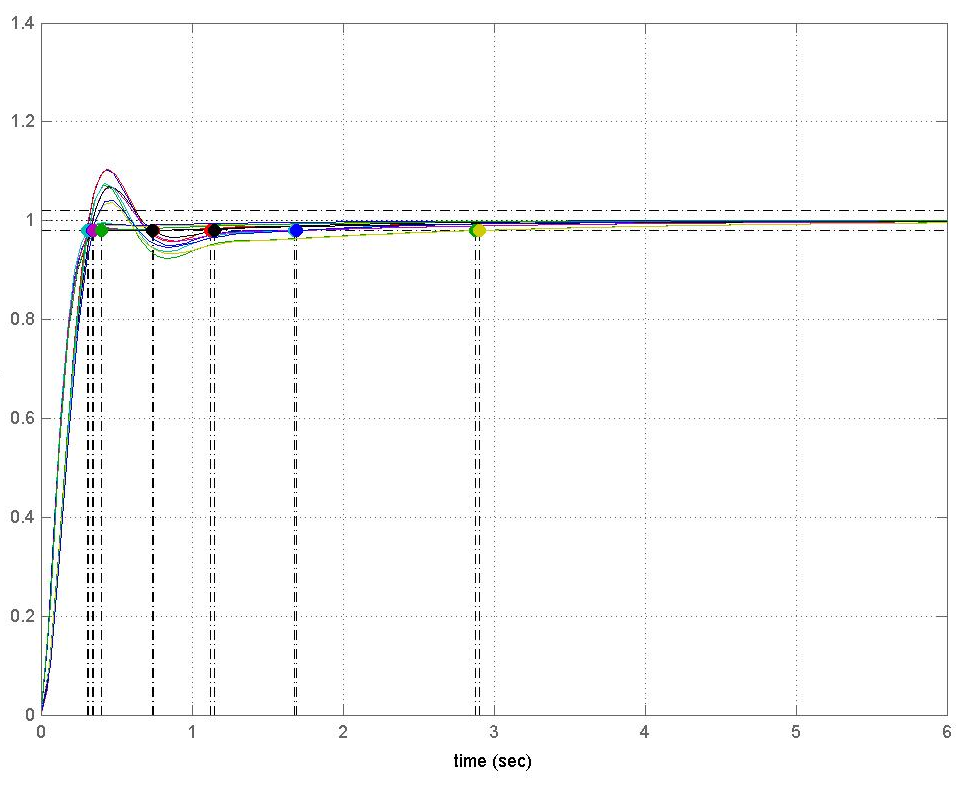
\includegraphics[scale=0.4]{screenshot.png}

Рассмотрим другой пример. Условия те же, но матрицы параметров отличаются.

\begin{equation*}
\begin{array}{lr}


%------------------------------------
A_1^0 = \left(\begin{array}{ccc}
0    &    1    &    0 \\
-14.1996    &    -6.08996    &    14.1996 \\
-2.96787    &    0    &    2.96787
\end{array}\right)\mbox{,} &
B_1^0 = \left(\begin{array}{c}
0 \\
-7.64812 \\
0
\end{array}\right)\mbox{;} \\

%------------------------------------
A_2^0 = \left(\begin{array}{ccc}
0    &    1    &    0 \\
-24.3236    &    -5.01533    &    24.3236 \\
-2.00206    &    0    &    2.00206
\end{array}\right)\mbox{,} &
B_2^0 = \left(\begin{array}{c}
0 \\
-12.3768 \\
0
\end{array}\right)\mbox{;} \\

%------------------------------------
A_3^0 = \left(\begin{array}{ccc}
0    &    1    &    0 \\
-43.0945    &    -5.43643    &    43.0945 \\
-2.72507    &    0    &    2.72507
\end{array}\right)\mbox{,} &
B_3^0 = \left(\begin{array}{c}
0 \\
-20.9305 \\
0
\end{array}\right)\mbox{;} \\

%------------------------------------
A_4^0 = \left(\begin{array}{ccc}
0    &    1    &    0 \\
-61.8141    &    -4.30745    &    61.8141 \\
-2.25735    &    0    &    2.25735
\end{array}\right)\mbox{,} &
B_4^0 = \left(\begin{array}{c}
0 \\
-22.0166 \\
0
\end{array}\right)\mbox{;} \\

%------------------------------------
A_5^0 = \left(\begin{array}{ccc}
0    &    1    &    0 \\
-68.4906    &    -1.5788    &    68.4906 \\
-1.90049    &    0    &    1.90049
\end{array}\right)\mbox{,} &
B_5^0 = \left(\begin{array}{c}
0 \\
-29.1617 \\
0
\end{array}\right)\mbox{;} \\

%------------------------------------
A_6^0 = \left(\begin{array}{ccc}
0    &    1    &    0 \\
-73.3721    &    -1.97372    &    73.3721 \\
-1.24783    &    0    &    1.24783
\end{array}\right)\mbox{,} &
B_6^0 = \left(\begin{array}{c}
0 \\
-36.5696 \\
0
\end{array}\right)\mbox{;} \\

%------------------------------------
A_7^0 = \left(\begin{array}{ccc}
0    &    1    &    0 \\
-85.9945    &    -4.94462    &    85.9945 \\
-1.65782    &    0    &    1.65782
\end{array}\right)\mbox{,} &
B_7^0 = \left(\begin{array}{c}
0 \\
-43.9964 \\
0
\end{array}\right)\mbox{;} \\

%------------------------------------
A_8^0 = \left(\begin{array}{ccc}
0    &    1    &    0 \\
-94.154    &    -8.35004    &    94.154 \\
-1.66214    &    0    &    1.66214
\end{array}\right)\mbox{,} &
B_8^0 = \left(\begin{array}{c}
0 \\
-47.8299 \\
0
\end{array}\right)\mbox{;} \\

%------------------------------------
A_9^0 = \left(\begin{array}{ccc}
0    &    1    &    0 \\
-110.563    &    -6.05252    &    110.563 \\
-0.610667    &    0    &    0.610667
\end{array}\right)\mbox{,} &
B_9^0 = \left(\begin{array}{c}
0 \\
-53.4986 \\
0
\end{array}\right)\mbox{;} \\

C_{i0} = \left(\begin{array}{ccc}
1 & 0 & 0 \\
0 & 1 & 0
\end{array}\right)\mbox{,} &
i \in \{1,2,\ldots,N\}.


\end{array}
\end{equation*}


Матрица усиления по алгоритмам \vref{alg:4/2} и \vref{alg:4/1}: $F = [-9.01~~-1]$. Итерационный алгоритм дал матрицу усиления $F=[-11.4~~-0.9]$.

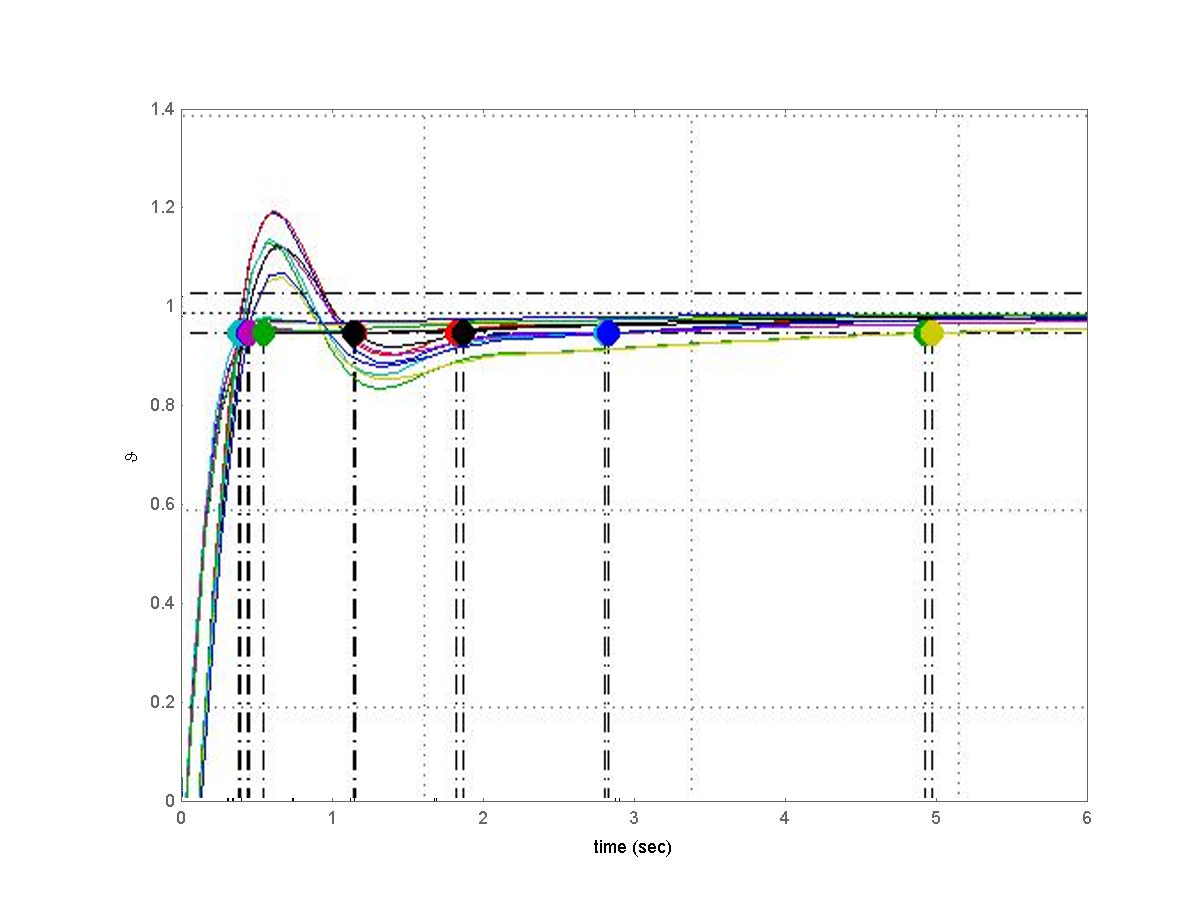
\includegraphics[scale=0.3]{screenshot2.png}

Рассмотрим вырожденный пример, на котором итерационный алгоритм расходится:

\begin{equation*}
\begin{array}{lr}


%------------------------------------
A_1^0 = \left(\begin{array}{ccc}
0    &    1    &    0 \\
12.4502    &    -3.71318    &    12.4502 \\
1.34787    &    0    &    1.34787
\end{array}\right)\mbox{,} &
B_1^0 = \left(\begin{array}{c}
0 \\
-1.06727 \\
0
\end{array}\right)\mbox{;} \\

%------------------------------------
A_2^0 = \left(\begin{array}{ccc}
0    &    1    &    0 \\
24.6718    &    -10.2687    &    24.6718 \\
2.60235    &    0    &    2.60235
\end{array}\right)\mbox{,} &
B_2^0 = \left(\begin{array}{c}
0 \\
-5.75874 \\
0
\end{array}\right)\mbox{;} \\

%------------------------------------
A_3^0 = \left(\begin{array}{ccc}
0    &    1    &    0 \\
34.7688    &    -7.92524    &    34.7688 \\
0.102741    &    0    &    0.102741
\end{array}\right)\mbox{,} &
B_3^0 = \left(\begin{array}{c}
0 \\
-11.3652 \\
0
\end{array}\right)\mbox{;} \\

%------------------------------------
A_4^0 = \left(\begin{array}{ccc}
0    &    1    &    0 \\
37.4861    &    -2.35985    &    37.4861 \\
2.86302    &    0    &    2.86302
\end{array}\right)\mbox{,} &
B_4^0 = \left(\begin{array}{c}
0 \\
-13.5763 \\
0
\end{array}\right)\mbox{;} \\

%------------------------------------
A_5^0 = \left(\begin{array}{ccc}
0    &    1    &    0 \\
39.7132    &    -10.9082    &    39.7132 \\
0.982049    &    0    &    0.982049
\end{array}\right)\mbox{,} &
B_5^0 = \left(\begin{array}{c}
0 \\
-16.5169 \\
0
\end{array}\right)\mbox{;} \\

%------------------------------------
A_6^0 = \left(\begin{array}{ccc}
0    &    1    &    0 \\
58.4972    &    -3.03661    &    58.4972 \\
0.370441    &    0    &    0.370441
\end{array}\right)\mbox{,} &
B_6^0 = \left(\begin{array}{c}
0 \\
-18.5588 \\
0
\end{array}\right)\mbox{;} \\

%------------------------------------
A_7^0 = \left(\begin{array}{ccc}
0    &    1    &    0 \\
66.6071    &    -6.62716    &    66.6071 \\
1.59545    &    0    &    1.59545
\end{array}\right)\mbox{,} &
B_7^0 = \left(\begin{array}{c}
0 \\
-20.3229 \\
0
\end{array}\right)\mbox{;} \\

%------------------------------------
A_8^0 = \left(\begin{array}{ccc}
0    &    1    &    0 \\
70.8975    &    -6.32684    &    70.8975 \\
2.97756    &    0    &    2.97756
\end{array}\right)\mbox{,} &
B_8^0 = \left(\begin{array}{c}
0 \\
-25.7138 \\
0
\end{array}\right)\mbox{;} \\

%------------------------------------
A_9^0 = \left(\begin{array}{ccc}
0    &    1    &    0 \\
87.8503    &    -3.14445    &    87.8503 \\
1.91167    &    0    &    1.91167
\end{array}\right)\mbox{,} &
B_9^0 = \left(\begin{array}{c}
0 \\
-35.2216 \\
0
\end{array}\right)\mbox{;} \\

C_{i0} = \left(\begin{array}{ccc}
1 & 0 & 0 \\
0 & 1 & 0
\end{array}\right)\mbox{,} &
i \in \{1,2,\ldots,N\}.
\end{array}
\end{equation*}

Итерационный алгоритм расходится. Алгоритм \vref{alg:4/2} дал же матрицу усиления $F = [-15.9567~~-1.002]$


% chapter 8: заключение
\chapter*{Заключение}
\addcontentsline{toc}{chapter}{Заключение}

Для линейных систем с непрерывным временем и шумами, зависящими от состояния и управления, получены необходимые и достаточные условия стабилизации, дающие параметрическое описание (параметризацию) всех линейных стабилизирующих управлений со статической обратной связью по выходу, которые обеспечивают экспоненциальную устойчивость в среднем квадратическом замкнутой системы. На основе этих результатов получены достаточные условия, с помощью которых нахождение матрицы усиления стабилизирующего управления сводится к задаче оптимизации при ограничениях в виде матричных линейных уравнений и неравенств.

Особенностью являлось то, что изначально поставленная задача была невыпукла, в следствие чего не имела удобных методов решения, основанных на достаточно проработанном математическом аппарате.\br

Были получены как алгоритмы робастной стабилизации, так и одновременной. Получен итерационный алгоритм, дающий удобный способ нахождения матриц усиления, с оговоркой на ограниченную применимость. Полученные результаты были успешно применены к решению задачи синтеза пассифицирующего управления с обратной связью по выходу, дан алгоритм решения.\br

Исследования проводились с помощью свободного программного обеспечения SciLab, синтаксического анализатора SciYalmip, являющегося свободной же реализацией известного пакета YALMIP, а также решателя CSDP\footnote{{\fontfamily{cmtt}\selectfont http://infohost.nmt.edu/$\sim$borchers/csdp.html}} под управлением операционной системы GNU/Linux. Успешность решения поставленных задач подтвердила достаточно высокое качество продуктов, поддерживаемых сообществом, сравнимое, а иногда и опережающее проприетарные аналоги.


% coding: utf-8
% --------------------------------------------------------------------------------------------------
% "Параметризация стабилизирующих управлений в стохастических системах с непрерывным временем", 2009
% : список литературы
% --------------------------------------------------------------------------------------------------

\addcontentsline{toc}{chapter}{Список использованной литературы}

\begin{thebibliography}{wlab}

\bibitem{TROF}
\emph{Crusius C.\,A.\,R., Trofino A}.
\newblock Sufficient LMI Conditions for Output Feedback Control Problems.
\newblock IEEE Trans. Automat. Control. 1999. V. 44. P. 1053–1057.

\bibitem{CDC}
\emph{Peaucelle D., Pakshin P.}
\newblock LQR parametrization of static output feedback gains for linear systems with Markovian switching and related robust stabilization and passification problems.

\bibitem{RUS}
\emph{Pakshin P., Solovyev S., Peaucelle D.}
\newblock Parametrization of stabilizing controllers for stochastic systems.

\bibitem{BOYD}
\emph{Boyd S., Ghaoui L.\,E., Feron E., Balakrishnan V.}
\newblock Linear Matrix Inequalities in System and Control Theory.
\newblock SIAM studies in applied mathematics; vol. 15, ISBN 0-89871-334-X, 1994.

\bibitem{CRUSIUS}
\emph{Crusius C.\,A.\,R.}
\newblock Formulac\~{a}o LMI para problemas de performance e robustez.
\newblock Master’s dissertation, Universidade Federal de Santa Catarina, EEL/UFSC Florian\'{o}polis, Brasil, 1996.

\bibitem{PERES}
\emph{Peres P.\,L.\,D., Geromel J.\,C., Souza S.\,R.}
\newblock Optimal $\mathcal{H}_2$ control by output feedback.
\newblock in \emph{Proc. Conf. Decision and Control}, Dec. 1993, pp. 102–107.

\bibitem{GLXKA}
\emph{Gadewadikar J., Lewis F.\,L., Xie L., Kucera V., Abu-Khalaf M.}
\newblock Parametrization of all stabilizing static state-feedback gains: Application to output-feedback design
\newblock Automatica, Vol.43. pp. 1597 - 1604, 2007.

\pagebreak

\bibitem{KM}
\emph{Kats I.\,Ya., Martynyk A.\,A.}
\newblock Stability and stabilization of nonlinear systems with random structures.
\newblock Taylor and Francis, London, 2002.

\bibitem{SIG}
\emph{Skeleton R.\,E., Iwasaki T., Grigoriadis K.\,M.}
\newblock A unified algebraic approach to linear control design.
\newblock Taylor and Francis, London, 1997.

\bibitem{PF}
\emph{Peaucelle D., Fradkov A.}
\newblock LMI conditions for robust adaptive control of LTI systems.
\newblock In \emph{IFAC Workshop on Adaptation and Learning in Control and Signal Processing}, St. Petersburg, August 2007. Paper
in \emph{Invited Session ''Passification-based Adaptive and Robust Control``}.

\bibitem{YAKUBOVICH}
\emph{Якубович В.\,А.}
\newblock Решение некоторых матричных неравенств, встречающихся в теории автоматического регулирования.
\newblock ДАН СССР. 1962. Т. 143 №6, с. 1304-1307

\bibitem{FRADKOV}
\emph{Фрадков А.\,Л., Андриевский Б.\,Р.}
\newblock Метод пассификации в задачах адаптивного управления, оценивания и синхронизации.
\newblock Автоматика и телемеханика, 2006. №11, С. 3-37.



\end{thebibliography}
 % +++

\chapter*{Пример реализации алгоритмов на языке SciLab}
\addcontentsline{toc}{chapter}{Приложение}

\lstset{language=Matlab,tabsize=4}
\lstinputlisting{appendix_code.m}


\end{document}
